\section{Applications} \label{applications}

Implementations of neural networks \ref{nn} (sometimes referred to as the black box) have been used for decades. The goal is to recommend visually similar images to those, which has user interacted with. Furthermore, this system can recommend advertisements which translate into revenue for the social platform. 

\begin{figure}[h]
    \centering
    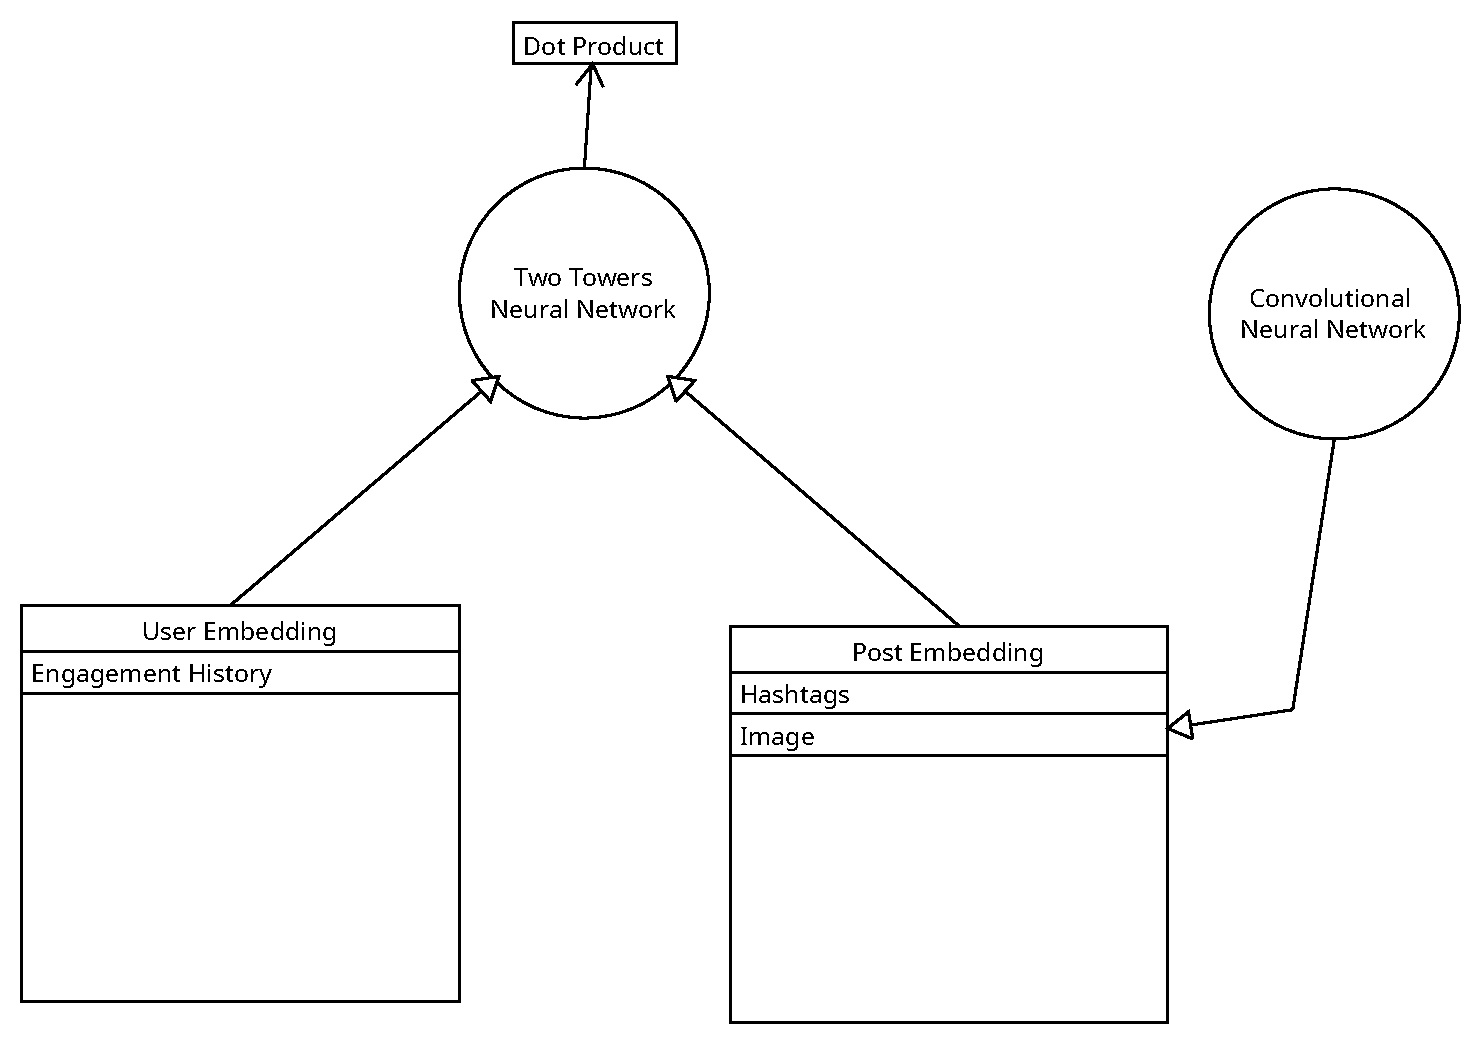
\includegraphics[width=0.7\linewidth]{Diagrams/architecture.pdf}
    \caption{Proposed architecture for content based image recommendation system}
    \label{fig:proposed-alogrithm}
\end{figure}

One of the main challenges in recommendation systems is recommending a new post to users, which hasn't been scored before. Such a problem is called ‘Cold Start' \ref{cold-start} problem. \cite{10373857} Same goes for recommending posts to a new user

\subsection{Content Based Filtering}\label{applications/content-based-filtering}

This type of filtering uses machine learning to make sure people are always seeing content that is the most interesting and relevant to them \cite{ig-new-content}


\subsection{Collaborative Filtering}\label{applications/collaborative-filtering}

To compare similarity of two accounts, this method calculates the cosine distance or dot product of two accounts. \cite{ig-explore} This way, users are filtered into groups of people with the same interests. After you have engaged with content from accounts of a certain group, you will be recommended more content from similar accounts. 

\begin{figure}[h]
    \centering
    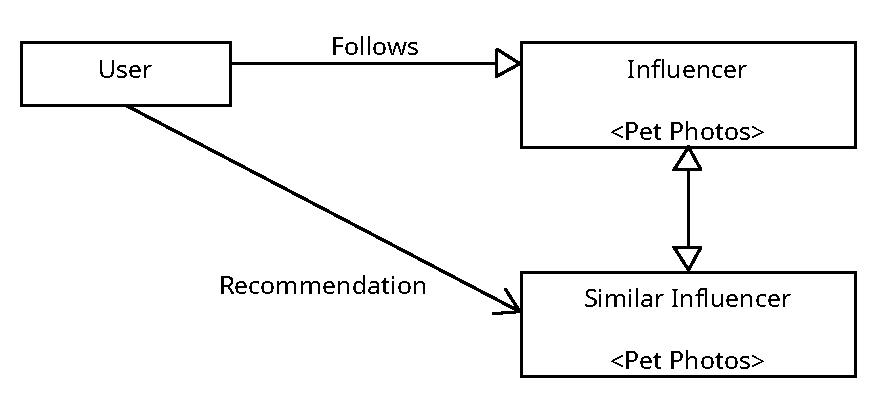
\includegraphics[width=0.7\linewidth]{Diagrams/collaborative-filtering.pdf}
    \caption{Example of account recommendation}
    \label{fig:collaborative-filtering-diagram}
\end{figure}